\documentclass[utf8]{beamer}

% This file is a solution template for:

% - Talk at a conference/colloquium.
% - Talk length is about 20min.
% - Style is ornate.

\mode<presentation>
{
  \usetheme{Warsaw}
  % or ...

  %\setbeamercovered{transparent}
  % or whatever (possibly just delete it)
}


\usepackage[english]{babel}

\usepackage[utf8]{inputenc}
% or whatever

\usepackage{times}
\usepackage[T1]{fontenc}
% Or whatever. Note that the encoding and the font should match. If T1
% does not look nice, try deleting the line with the fontenc.


\title{A flexible Prolog interpreter in Python}

\author{Carl Friedrich Bolz}
% - Give the names in the same order as the appear in the paper.
% - Use the \inst{?} command only if the authors have different
%   affiliation.

\institute[Heinrich-Heine-Universität Düsseldorf]
{
  Institut für Informatik\\
  Heinrich-Heine-Universität Düsseldorf
}

\date{24. Workshop der GI-Fachgruppe Programmiersprachen und Rechenkonzepte, 4. Mai 2007}
% - Either use conference name or its abbreviation.
% - Not really informative to the audience, more for people (including
%   yourself) who are reading the slides online


% If you have a file called "university-logo-filename.xxx", where xxx
% is a graphic format that can be processed by latex or pdflatex,
% resp., then you can add a logo as follows:

\pgfdeclareimage[height=0.5cm]{pypy-logo}{image/py-web.png}
\logo{\pgfuseimage{pypy-logo}}



% Delete this, if you do not want the table of contents to pop up at
% the beginning of each subsection:
%\AtBeginSubsection[]
%{
%  \begin{frame}<beamer>
%    \frametitle{Outline}
%    \tableofcontents[currentsection,currentsubsection]
%  \end{frame}
%}


% If you wish to uncover everything in a step-wise fashion, uncomment
% the following command: 

%\beamerdefaultoverlayspecification{<+->}


\begin{document}

\begin{frame}
  \titlepage
\end{frame}

%\begin{frame}
%  \frametitle{Outline}
%  \tableofcontents
  % You might wish to add the option [pausesections]
%\end{frame}


% Structuring a talk is a difficult task and the following structure
% may not be suitable. Here are some rules that apply for this
% solution: 

% - Exactly two or three sections (other than the summary).
% - At *most* three subsections per section.
% - Talk about 30s to 2min per frame. So there should be between about
%   15 and 30 frames, all told.

% - A conference audience is likely to know very little of what you
%   are going to talk about. So *simplify*!
% - In a 20min talk, getting the main ideas across is hard
%   enough. Leave out details, even if it means being less precise than
%   you think necessary.
% - If you omit details that are vital to the proof/implementation,
%   just say so once. Everybody will be happy with that.

\section{What is Pyrolog?}

\begin{frame}
  \frametitle{Pyrolog}

  \begin{itemize}
  \item
    Pyrolog is a Prolog interpreter written in Python
  \item
    want to compile it to get interesting performance
  \item
    translation tool-chain part of the PyPy project
  \item
    Python itself is too dynamic to be translatable to other languages, need a subset
  \item
    RPython (``Restricted Python'') is a subset of Python translatable to other
    languages
  \item
    RPython is designed to be significantly faster than regular Python
  \end{itemize}
\end{frame}

\section{The PyPy Approach to VM Construction}
\subsection{Overview}
\begin{frame}
  \frametitle{What is PyPy?}
  \begin{itemize}
  \item
    started as a Python VM implementation in Python
  \item
    most important part: translation tool-chain for RPython
  \item
    is becoming a general environment for writing interpreters (JavaScript, Prolog started)
  \item
    Open Source project (MIT license)
  \item
    received EU funding for 2.5 years
  \end{itemize}

\end{frame}

\subsection{Motivation}
\begin{frame}
  \frametitle{VMs are still hard}
  Hard to reconcile:

  \begin{itemize}
  \item
    flexibility
  \item
    maintainability
  \item
    performance (needs dynamic compilation techniques)
  \end{itemize}
  Especially with limited resources (like Open Source projects, research projects)
\end{frame}


\begin{frame}
  \frametitle{The Python case}
  CPython (the reference implementation) is a straightforward, portable VM.

  \begin{itemize}
  \item
    Pervasive decisions: reference counting, global lock \dots
  \item
    No dynamic compilation
  \end{itemize}
  \pause
  \begin{block}{
    Extensions:}
    \begin{itemize}
    \item
      \alert{Stackless} (unlimited recursion, coroutines, green threads)
    \item
      \alert{Psyco} (run-time specializing compiler)
    \item
      \alert{Jython}, \alert{IronPython}
    \end{itemize}
  \end{block}
\end{frame}



\begin{frame}
  \frametitle{The Prolog case (i)}
  \begin{itemize}
  \item
    problem mitigated by the fact that Prolog the language does not change
  \item
    the core of Prolog is very simple (at least compared to Python)
  \item
    a lot of implementations out there
  \item
    well-tuned mature C implementations (Sicstus, XSB, SWI, GNU-Prolog)
  \item
    on CLR (P\#) and JVM (Prolog Café, tuProlog)
  \end{itemize}
\end{frame}

\begin{frame}
  \frametitle{The Prolog case (ii)}
  \begin{block}{mature C implementations}
    \begin{itemize}
    \item
      interfacing with libraries is tedious
    \item
      changing the language to experiment is hard
    \item
      often extensions to core Prolog, incompatible between each other
    \end{itemize}
  \end{block}
  \pause
  \begin{block}{implementations on CLR and JVM}
    \begin{itemize}
    \item
      interfacing with libraries of the platform mostly easy
    \item
      no extensions to core Prolog (like tabling, coroutines, constraints)
    \item
      slow, compared to good C implementations
    \end{itemize}
  \end{block}
\end{frame}



\subsection{Approach}
\begin{frame}
  \frametitle{PyPy's Approach}
    \alert{Goal:} generate VMs from a single high-level description of the
     language, in a retargettable way.
  \begin{itemize}
  \item
    Write an  interpreter for a dynamic language (Python, Prolog, JavaScript,
    whatever) in a high-level language (Python)
  \item
    Leave out low-level details
  \item
    Favour simplicity and flexibility
  \item
    Define a mapping to low-level targets
  \item
    Generate VMs from the interpreter
  \end{itemize}
\end{frame}


\begin{frame}
  \frametitle{Mapping to low-level targets}
  \begin{itemize}
  \item
    Mechanically translate the interpreter to multiple
    lower-level targets
    \begin{itemize}
    \item C-like
    \item .NET
    \item Java
    \end{itemize}
  \pause
  \item
    Insert low-level aspects into the code as required by
    the target
    \begin{itemize}
    \item object layout
    \item memory management
    \end{itemize}
  \pause
  \item
    Optionally insert new pervasive features not expressed
    in the source
    \begin{itemize}
    \item continuations, ``micro-threads''
    \item dynamic compilation
    \end{itemize}
  \end{itemize}
\end{frame}



\begin{frame}
  \frametitle{Translation Aspects (i)}
  Features not present in the source can be added during translation:
  \begin{itemize}
  \item
    \alert{memory management}: use different GC strategies (Boehm collector, custom mark-n-sweep)
  \item
    \alert{Stackless transformation}: allows program to control its stack (continuations, \dots)
  \end{itemize}
\end{frame}


\begin{frame}
  \frametitle{Translation Aspects (ii)}
  A \alert{JIT compiler} as a translation aspect
  \begin{itemize}
  \item
    Transform the interpreter into a JIT compiler, using partial evaluation and
    specialization techniques
  \item
    Some hints in the interpreter source needed
  \item
    Current prototype applied to Python interpreter gives impressive speedups
  \end{itemize}
\end{frame}

\section{The Prolog interpreter}
\subsection{Interpreter}
\begin{frame}
  \frametitle{Prolog Interpreter Implementation}
  \begin{itemize}
  \item
    naive, very simple interpreter
    \begin{itemize}
    \item uses "structure copying"
    \item interprets Prolog terms directly, no bytecode
    \end{itemize}
  \item
    uses continuation passing style inspired by BinProlog
  \item
    implements large parts of the ISO standard (some builtins missing)
  \end{itemize}
\end{frame}


\begin{frame}
  \frametitle{Builtins}
  \begin{itemize}
  \item
    builtins implemented in Python
  \item
    easy to add new ones to interface with libraries
  \item
    application-specific builtins
  \item
    examples:
    \begin{itemize}
    \item functions to download and analyze webpages
    \item an imperative hashmap
    \end{itemize}
  \end{itemize}
\end{frame}


\begin{frame}
  \frametitle{Interpreter Facts}
  \begin{itemize}
  \item
    2500 lines of Python code in total
  \item
    700 of those are for builtins
  \item
    after translation to C: 14000 lines of C code
  \item
    part of the PyPy distribution at:
    \texttt{http://codespeak.net/pypy}
  \end{itemize}
\end{frame}


\subsection{Performance}
\begin{frame}
  \frametitle{Performance (i)}
  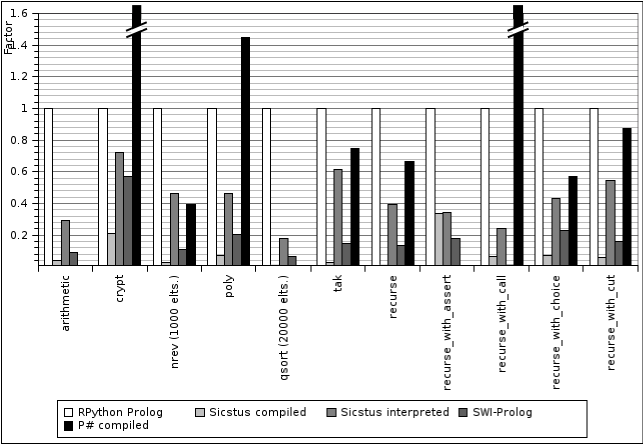
\includegraphics[scale=0.4]{image/bench.png}
\end{frame}


\begin{frame}
  \frametitle{Performance (ii)}
  \begin{itemize}
  \item
    performance is quite bad compared to tuned C implementations
  \item
    performance is pretty good compared to Java and .NET implementations
  \item
    surprising, since those are often based on the WAM
  \item
    maybe the WAM model does not match these VMs very well?
  \end{itemize}
\end{frame}


\section*{Summary}
\subsection*{Summary}
\begin{frame}
  \frametitle{Summary}

  \begin{itemize}
  \item
    Very simple Prolog interpreter in RPython can compete with interpreters on the JVM, CLR
  \item
    Interpreter implementation eased by use of a high-level language
  \item
    Low-level details abstracted away but re-inserted later
  \end{itemize}
\end{frame}

\subsection*{Outlook}
\begin{frame}
  \frametitle{Outlook}
  \begin{itemize}
  \item
    complete the set of builtins
  \item
    tight language integration between Prolog and Python
  \item
    apply the dynamic compiler generator to the Prolog interpreter
  \end{itemize}
\end{frame}

\begin{frame}
  \frametitle{Questions?}
  \begin{center}
  
\includegraphics[scale=0.5]{image/py-web.png}
  
  \texttt{http://codespeak.net/pypy}
  \end{center}
\end{frame}


\begin{frame}
  \frametitle{Backup slides}
  \dots
\end{frame}

\begin{frame}
  \frametitle{Translation Steps}
  \begin{columns}[c]
  \begin{column}{5cm}
    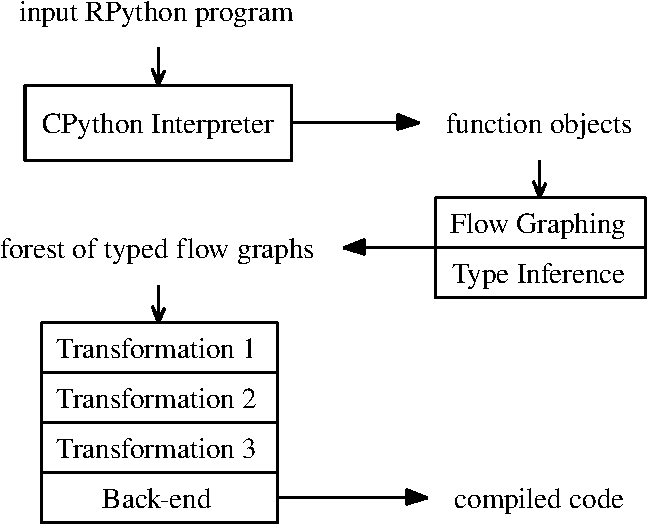
\includegraphics[width=5cm]{image/arch.pdf}
  \end{column}
  \begin{column}{7cm}
  \begin{itemize}
    \item
      Generate flow graphs from the RPython program
    \item
      Peform global type inference on the flow graphs
    \item
      Transform flow graphs through several steps until they match the level of
      the target environment
    \item
      Weave in translation aspects in the process
  \end{itemize}
  \end{column}
  \end{columns}
\end{frame}

\begin{frame}
  \frametitle{Title}
  \begin{itemize}
  \item
  \end{itemize}
\end{frame}



\end{document}


